\documentclass[12pt,twoside,openright,a4paper,english,brazil,sumario=tradicional]{abntex2}
\usepackage[utf8]{inputenc}
\usepackage[T1]{fontenc}
\usepackage{indentfirst}
\usepackage{color}
\usepackage{graphicx}
\usepackage{microtype}
\usepackage[brazilian,hyperpageref]{backref}
\usepackage[alf]{abntex2cite}
\usepackage{multicol}
\usepackage{multirow}
\usepackage{enumitem}
\usepackage{amsfonts}
\usepackage{amssymb}
\usepackage{listings}
\usepackage{tikz-uml}

\usepackage{uarial}
\renewcommand{\familydefault}{\sfdefault}
\usepackage{blindtext}

\graphicspath{{../images/}}

\renewcommand{\backrefpagesname}{Citado na(s) página(s):~}
\renewcommand{\backref}{}
\renewcommand*{\backrefalt}[4]{
	\ifcase #1 %
		Nenhuma citação no texto.%
	\or
		Citado na página #2.%
	\else		Citado #1 vezes nas páginas #2.%
	\fi}%

\titulo{Módulo de pré-vizualização para a ferramenta CGT - Ceará Game Tools}
\author{Joel Xavier Rocha\thanks{\texttt{joelxr@gmail.com}}}
\orientador{Prof. Dr. Carlos Hairon Ribeiro Gonçalves}
\local{Fortaleza}
\data{2015}
\instituicao{
  Instituto Federal de Ciência, Educação e Tecnologia do Ceará
  \par
  Engenharia de Computação}
\tipotrabalho{Monografia}
\preambulo{Trabalho de conclusão de curso apresentado à banca examinadora do Instituto Federal de Educação, Ciência e Tecnologia do Ceará para obtenção do grau de bacharel em Engenharia de Computação sob a orientação do Prof. Dr. Carlos Hairon Ribeiro Gonçalves.}
\definecolor{blue}{RGB}{41,5,195}
\makeatletter
\hypersetup{
   pdftitle={\@title},
	 pdfauthor={\@author},
   pdfsubject={Trabalho de conclusão de curso},
   pdfcreator={pdfLaTeX},
   pdfkeywords={abnt}{latex}{abntex}{abntex2}{trabalho científico},
   colorlinks=true,
   linkcolor=blue,
   citecolor=blue,
   filecolor=magenta,
   urlcolor=blue,
   bookmarksdepth=4
}
\makeatother
\setlength{\parindent}{1.3cm}
\setlength{\parskip}{0.2cm}
\makeindex

\begin{document}
\selectlanguage{brazil}
\frenchspacing
\imprimircapa
\imprimirfolhaderosto*

% \begin{fichacatalografica}
%     \includepdf{fig_ficha_catalografica.pdf}
% \end{fichacatalografica}

% \includepdf{folhadeaprovacao_final.pdf}

\begin{agradecimentos}

\end{agradecimentos}

\setlength{\absparsep}{18pt}
\begin{resumo}
O crescimento da industria de jogos em diversas áreas - como entretenimento e educação - torna necessário a elaboração de ferramentas que possibilitem a criação destes de forma simples, fácil e objetiva. Por esta razão, o projeto \emph{Ceará Game Tools} (CGT), tem como objetivo possibilitar isso aos usuários que não conhecem os meios e as técnicas envolvidas na criação de jogos.

Então, é proposto nesse trabalho, melhorias importantes para a ferramenta CGT, principalmente, a pré visualização do jogo que está sendo construído e também dos seus objetos.

\vspace{\onelineskip}
\noindent
\textbf{Palavras-chave}: CGT, ferramenta;
\end{resumo}

\pdfbookmark[0]{\listfigurename}{lof}
\listoffigures*
\cleardoublepage

\pdfbookmark[0]{\listtablename}{lot}
\listoftables*
\cleardoublepage

\pdfbookmark[0]{\contentsname}{toc}
\tableofcontents*
\cleardoublepage

\textual

\chapter{Introdução} % Ryllari
\label{chap:introducao}

% introduzindo sobre o que é o trabalho
Neste trabalho, é apresentado problemas existentes e pontos de melhorias na primeira versão da ferramenta de construção de jogos do projeto CGT (\texttt{ferramenta 1.0}). Bem como, de que modo essas questões foram tratadas e implementadas na segunda versão (\texttt{ferramenta 2.0}). A nova versão da ferramenta tem como objetivo melhorar o processe de criação de jogos e tornar essa tarefa mais intuitiva para o usuário final.

\section{O projeto CGT}
% Descrição/apresentação do projeto CGT
O projeto CGT que surgiu para tornar possível a qualquer pessoa a criação de jogos, assim como é explicado no trabalho \cite{monografia:aquino}, vem sido desenvolvido há cerca de um ano e possibilita a construção de jogos eletrônicos por qualquer pessoa, não sendo necessário conhecimentos em programação ou nas técnicas de criação de jogos. De foma fácil, simples e prática, a ferramenta, atende a necessidade da maior parte dos usuários, podendo produzir jogos de vários temas e para diversos fins, desde entretenimento a educação, por exemplo. Assim como, é proposto no \emph{website} do projeto.

\begin{citacao}
O projeto Ceará Game Tools tem como objetivo oferecer uma ferramenta para a construção de jogos. Em suma, qualquer um poderá criar seu próprio jogo utilizando componentes \emph{drag-and-drop} e os configurando. \cite{website:projeto-cgt}
\end{citacao}

\subsection{Vínculo com o CNPQ} % Pegar informações com Ryllari
O CNPQ\footnote{Centro Nacional de desenvolvimento científico e tecnológico.}

\subsection{Os módulos desenvolvidos para o projeto}
% ferramenta de construção de jogos
O projeto é composto por módulos - mostrados na tabela \ref{table:modules} - onde um deles é a \texttt{a ferramenta} que é objeto de estudo para este trabalho. O objetivo desta ferramenta é implementar toda a interação com o usuário e ser responsável por apresentar o jogo para o usuário final no momento da sua criação. Tudo isso de forma intuitiva, simples e prática.

\begin{table}

\end{table}

\begin{table}[h]
\centering
\begin{tabular}{ | l | p{10cm} | }
    \hline
    Módulos & Descrição \\ \hline
    \texttt{core} & Contém os objetos essenciais para o projeto. \\
    \texttt{desktop} & Responsável por possibilitar a execução do jogo no computador. \\
		\texttt{ferramenta} & Corresponde ao módulo objeto de estudo deste trabalho que possibilita a criação do jogo. \\
		\texttt{android} & Permite exportar o jogo para execução dos dispositivos \emph{Android}. \\
		\texttt{ios} & Permite exportar o jogo para execução dos dispositivos \emph{iOS}. \\
    \hline
\end{tabular}
\caption{Módulos existentes no projeto CGT }
\label{table:modulos}
\end{table}

\section{Introdução ao problema}
% Como foi feita a identificação dos problemas? por que? por e para quem?
A identificação dos problemas e pontos de melhoria para a ferramenta foram percebidos, principalmente, atráves do uso e estão relacionados a interação com o usuário final e a percepção deste com o jogo em produção.

% principal problema
A \texttt{ferramenta 1.0} é bastante robusta e atende bem com o propósito de criar os objetos que compõem o jogo e, eventualmente, produzir o jogo em forma de aplicação para a plataforma destino. Entretanto, a mesma carece em fornecer algum \emph{feedback} no momento da criação, obrigando ao usuário a sempre executar o jogo para poder perceber atributos essenciais dos objetos, tais como: a posição, o tamanho, a textura entre outros. Por exemplo, as posições de um objeto no jogo são configuradas, entretanto, o usuário precisa executar o jogo para poder visualizar o que configurou, na imagem \ref{fig:intro-problema-1} pode-se ver que há duas janelas abertas, uma da ferramenta e outra do jogo em execução. Com isso, os seguintes questionamentos podem ser feitos: Para todo objeto, é preciso executar e ver como ficou a configuração? Quais os outros objetos que isso acontece? Quais as outras propriedades que isso acontece?

\begin{figure}[htb]
\label{fig:intro-problema-1}
\centering
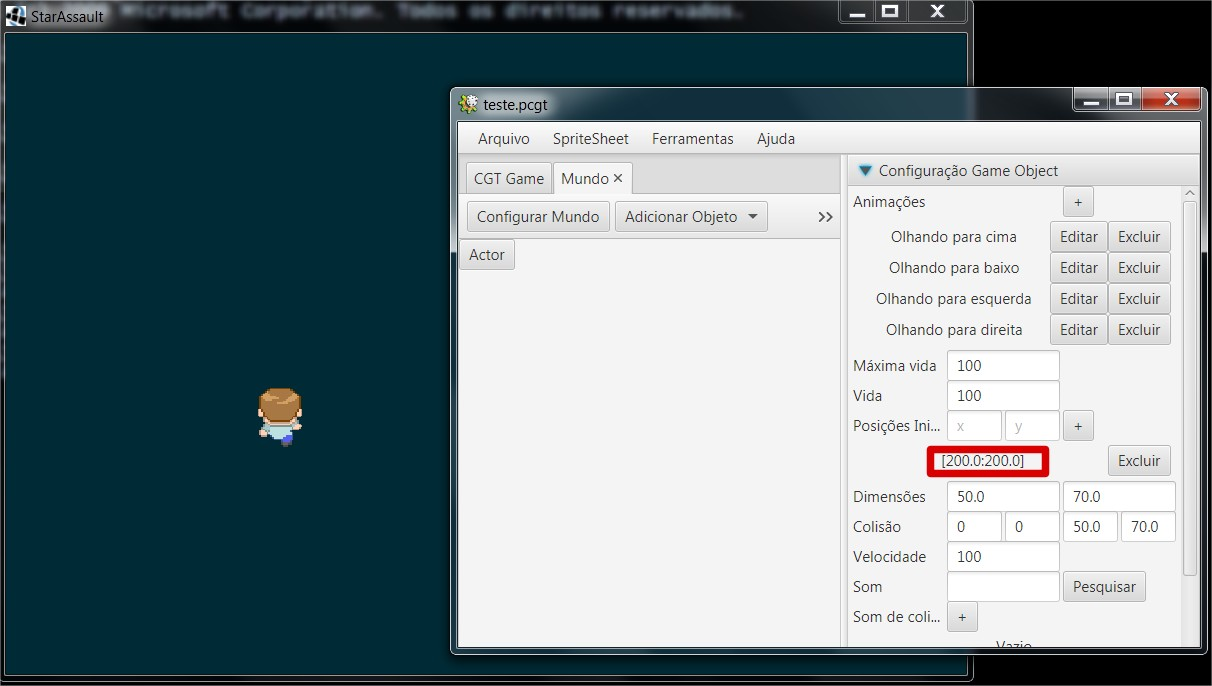
\includegraphics[width=0.7\textwidth]{images/problema-1.jpg}
\caption{Problema de pré-visualização na \texttt{ferramenta 1.0}.}
\end{figure}

% mais problemas
Além disso, os controles que fazem parte da primeira versão da ferramenta, tornam, na maioria das vezes, oneroso o processo de configuração dos objetos. Por exemplo, a configuração das animações que possui um objeto. É necessário criar as animações olhando no \emph{spritesheet}\footnote{Imagem que contém todas as faces de um objeto no jogo.} do objeto e preenchendo campos de texto com o valor da linha e coluna do \emph{sprite} correspondente a animação configurada (ver imagem \ref{fig:intro-problema-2}).

\begin{figure}[htb]
\label{fig:intro-problema-2}
\centering
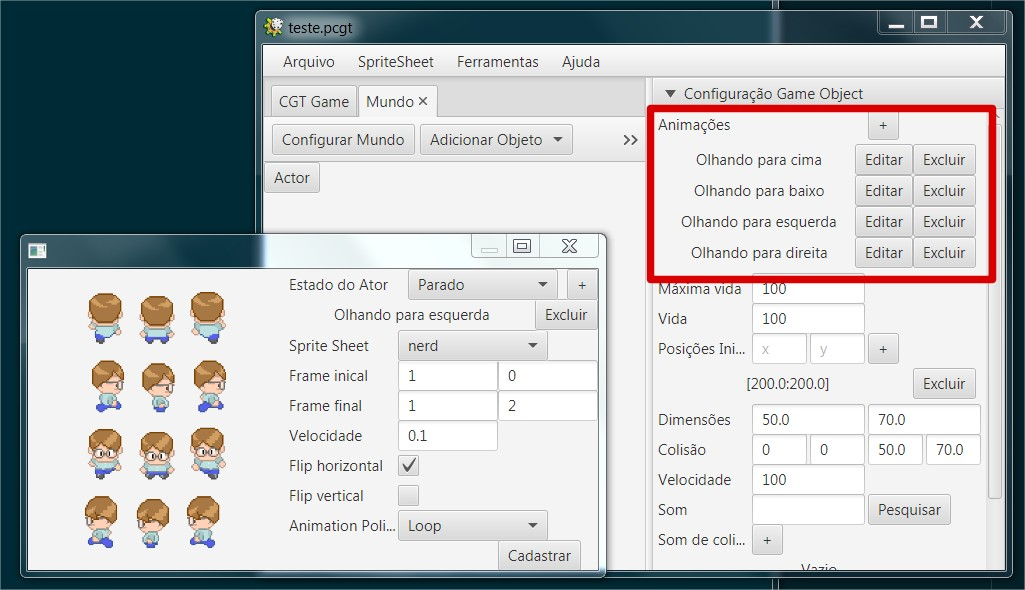
\includegraphics[width=0.7\textwidth]{images/problema-2.jpg}
\caption{Problema com os controles na configuração de uma animção na \texttt{ferramenta 1.0}.}
\end{figure}

Os problemas encontrados na \texttt{ferramenta 1.0} foram a motivação para esse trabalho e serão descritos detalhadamente no capitulo \ref{chap:problemas}.

\section{Disposição do documento}
% Falar sobre cada parte do documento e qual o objetivo de cada uma
Este documento está dividido basicamente em três partes que são:
\begin{description}
	\item[Definir o problema] Mostrado no capítulo \ref{chap:problemas}, como já dito anteriormente, tem como objetivo enumerar detalhadamente os problemas e pontos de melhoria encontrados na \texttt{ferramenta 1.0}. Dessa forma, prepara-se uma lista das principais funcionalidades que farão parte da nova versão da ferramenta.
	\item[Proposta de melhorias] Corresponde ao capítulo \ref{chap:melhorias} que visa propor soluções para as questões encontradas anteriormente e explicar como foram alcançadas.
	\item[Análise dos resultados] É um estudo de caso, mostrado no capítulo \ref{chap:caso}, com a nova versão da ferramenta, onde busca-se comparar o tempo de criação de jogo, a facilidade de uso e a quantidade de esforço necessário para configurar.
\end{description}

\chapter{Problema}
\label{chap:problemas}
% breve descrição do problema do preview
A ferramenta de construção de jogos do projeto CGT é robusta e atende aos objetivos propostos. Contudo, ela possui lacunas quando se trata da interação humano-computador (IHC), é possível listar:

\begin{alineas}
	\item A falta de pré-vizualização dos objetos contidos no jogo, que torna difícil a percepção do usuário, obrigando-o a sempre executar o jogo para observar as configurações que foram feitas;
	\item Os controles não são claros e, assim, produzir um jogo pode acabar sendo uma experiência onerosa e repleta de configurações repetitivas.
\end{alineas}

Com esses itens em mente, a seguir, é mostrado como construir um jogo de exemplo na primeira versão da ferramenta e, a partir daí, quais problemas e melhorias são notados.

\section{Objetos de um jogo}
\label{sec:objetos}

A fim de enumerar os problemas e melhorias, torna-se necessário construir um jogo com a \texttt{ferramenta 1.0} e, para fazê-lo, deve-se conhecer os objetos que existem e como devemos configura-los. Então, a seguir, há uma lista dos possíveis objetos que podem compor um jogo:

\begin{itemize}
	\item Mundo,
	\item Ator,
	\item Inimigo,
	\item Opositor,
	\item Bônus,
	\item Projétil,
	\item Tela,
	\item Botão de tela,
	\item Vida de um objeto e
	\item Munição de um objeto.
\end{itemize}

Na secção \ref{sec:dificuldades}, será criado um jogo de exemplo na ferramenta, a fim de mostrar os problemas e pontos de melhoria percebidos. O manual da \texttt{ferramenta 2.0} está na parte de anexos e pode ser consultado para entender como funciona a criação de cada objeto listado.

\section{Dificuldades encontradas}
\label{sec:dificuldades}
% detalhar dificuldades com figuras da ferramenta 1.0, fazer um jogo de exemplo que será usado posteriormente

\section{Game JAM} % Ryllari

\chapter{Descrição das melhorias} % Joel
\label{chap:melhorias}
\section{Pontos de melhoria}
\section{Detalhes da implementação do novo módulo}
\subsection{Métodos e ferramentas}
\subsection{Descrição do módulo}

\chapter{Estudo de caso}
\label{chap:caso}
\section{Análise dos resultados}
\section{Comparativo}
\section{Jogo exemplo}
\section{Projeto de extensão}

\chapter{Conclusão e trabalhos futuros}
\label{chap:conclcsao}

\postextual
\bibliography{references}

\begin{apendicesenv}
\partapendices
\chapter{Diagramas UML}
\label{chap:diagramas}

\section{Diagrama de classes}
No diagrama de classes a seguir, temos a notação UML para as classes do módulo \texttt{ferramenta} do projeto CGT que estão localizadas dentro do pacote \texttt{br.edu.ifce.cgt.application}.

\begin{figure}[h]
\label{fig:diagrama-classes}
\centering
\begin{tikzpicture}
\begin{umlpackage}{vo}
\umlinterface{DrawableObject}{}
{
	getObject() : T \\
	setObject(obj : T) : void \\
	getPane() : Node \\
	drawObject() : void \\
	drawConfigurationPanel() : void \\
	onCreate() : void \\
	onStart() : void \\
	destroy() : boolean }
\umlclass[x=8,y=0]{AbstractDrawableObject}
{
	- object : T \\
	- drawableObjectPane : Pane \\
	- drawConfigurationPanel : Pane
}
{
	getDrawableObjectPane() : Pane \\
	getDrawableConfigurationsPane() : Pane \\
	updateDrawPane(node : Node) : void \\
	updateConfigPane(node : Node) : void \\
	updateConfigPane(pane : Pane) : void
}
\umlclass[x=0,y=-6]{CGTProjectDrawable}
{
	- size : Rectangle \\
	- projectPane : ConfigProjectPane
}{}
\umlclass[x=8,y=-6]{CGTGameObjectDrawable}
{
	- gameObjectTitledPane : GameObjectPane \\
	- worldName : String \\
	- bounds : Rectangle \\
	- collision : Rectangle \\
	- preview : Draggable
}
{}
\umlclass[x=0,y=-9]{CGTGameActorDrawable}{}{}
\umlclass[x=8,y=-10]{CGTGameEnemyDrawable}{}{}
\umlclass[x=0,y=-11]{CGTGameOppositeDrawable}{}{}
\umlclass[x=8,y=-12]{CGTGameBonusDrawable}{}{}
\umlclass[x=0,y=-13]{CGTGameProjectitleDrawable}{}{}
\umlclass[x=8,y=-14]{CGTGameScreenDrawable}{}{}
\umlclass[x=0,y=-15]{CGTButtonScreenPreview}{}{}
\umlclass[x=8,y=-16]{CGTLifeBarDrawable}{}{}
\umlclass[x=0,y=-17]{HUDComponetDrawable}{}{}
\umlclass[x=8,y=-18]{DrawableObjectTreeCellImpl}{}{}
%\umlimpl{DrawableObject}{AbstractDrawableObject}
%\umlimpl{AbstractDrawableObject}{CGTProjectDrawable}
%\umlimpl{AbstractDrawableObject}{CGTGameObjectDrawable}
%\umlimpl{CGTGameObjectDrawable}{CGTGameActorDrawable}
%\umlimpl{CGTGameObjectDrawable}{CGTGameEnemyDrawable}
%\umlimpl{CGTGameObjectDrawable}{CGTGameOppositeDrawable}
%\umlimpl{CGTGameObjectDrawable}{CGTGameBonusDrawable}
%\umlimpl{CGTGameObjectDrawable}{CGTGameProjectitleDrawable}
\end{umlpackage}
\end{tikzpicture}
\caption{Diagrama de classes UML para o módulo implementado.}
\end{figure}

\end{apendicesenv}

\begin{anexosenv}
\partanexos
\chapter{Manual da ferramenta}

\chapter{Código fonte}
\end{anexosenv}
\phantompart
\printindex
\end{document}
